% \iffalse meta-comment
%
% Copyright (C) 2019 by Yi Liu <me@yliu.io>
% -----------------------------------------------------------
%
% This file may be distributed and/or modified under the conditions of
% the LaTeX Project Public License, either version 1.3c of this license
% or (at your option) any later version. The latest version of this
% license is in:
%
% http://www.latex-project.org/lppl.txt
%
% and version 1.3c or later is part of all distributions of LaTeX
% version 2006/05/20 or later.
%
% \fi
%
% \iffalse
%<*driver>
\ProvidesFile{latexalpha2.dtx}
%</driver>
%<package>\NeedsTeXFormat{LaTeX2e}
%<package>\ProvidesPackage{latexalpha2}
%<*package>
  [2019/03/05 v1.1 latexalpha2]
%</package>
%
%<*driver>
\documentclass{ltxdoc}
\usepackage{latexalpha2}
\usepackage{amsmath}
\usepackage{etoolbox}
\usepackage{url}
\usepackage{spverbatim}
\usepackage{metalogo}
\makeatletter
\preto{\@verbatim}{\topsep=0pt \partopsep=0pt \vspace{10pt}}
\makeatother
\setlength\parindent{0pt}
\def\backslash{\char`\\}
\EnableCrossrefs
\CodelineIndex
\OnlyDescription
\begin{document}
  \DocInput{latexalpha2.dtx}
\end{document}
%</driver>
% \fi
%
% \GetFileInfo{latexalpha2.dtx}
% \title{The \textsf{latexalpha2} package\thanks{This document
%   corresponds to \textsf{latexalpha}~\fileversion,
%   date~\filedate.}}
% \author{Yi Liu\thanks{Personal website: \texttt{https://yliu.io}.}\\me@yliu.io}
% \date{\filedate}
% \maketitle
%
% \section{Introduction}
%
% \textsf{latexalpha2} is a \LaTeX~package that allows you to embed and execute your Wolfram Language (Mathematica) source codes in a \LaTeX~document. When the document is compiled, the computation results will be inserted into the compiled file. For example,
% \begin{verbatim}
%   $$ \wolfram{LaplaceTransform[t^4 Sin[t],t,s]} $$
% \end{verbatim}
% gives the Laplace transform of $t^4\sin t$ and generates
%   $$ \wolfram{LaplaceTransform[t^4 Sin[t],t,s]}. $$
% It is also quite easy to generate plots or animations with this package. Moreover, all the embedded codes can be executed either locally or on the cloud. In addition, you can also use Mathics\footnote{\url{http://mathics.github.io}} (a free alternative to Mathematica) for computations.
%
% The main features of the package are somewhat similar to \texttt{SageTeX}\footnote{\url{https://ctan.org/pkg/sagetex}}, but here we use Wolfram Language (Mathematica) instead of Sage.
%
% If you have any questions or comments, you are welcome to raise issues or pull requests through the Github repository for this package\footnote{\url{https://github.com/stevenliuyi/latex-alpha2}}. For now, \textsf{latexalpha2} only supports Unix-like systems.
%
% This package is \textit{not} endorsed by or affiliated with Wolfram Research, Inc. in any way.
%
% \section{Installation}
%
% The Wolfram Language codes are executed using the WolframScript interpreter\footnote{\url{https://www.wolfram.com/wolframscript}}. So please make sure that WolframScript is properly installed before using \textsf{latexalpha2}. If you'd like to run your codes on cloud, please authenticate first:
%
% \begin{verbatim}
%   wolframscript -authenticate
% \end{verbatim}
%
% Alternatively, if you are using Mathics for computations, please make sure that Mathics is properly installed. Please refer to the Mathics installation guide\footnote{\url{https://github.com/mathics/Mathics/wiki/Installing}} for more information.
%
% When compiling your document, \LaTeX~must be invoked with the \texttt{-shell-escape} flag in order to run either WolframScript or Mathics. Currently, this package is only tested with pdf\LaTeX~and~\XeLaTeX. After putting \texttt{\backslash usepackage\string{latexalpha2\string}} in the preamable of your document, you can compile the file as:
%
% \begin{verbatim}
%   pdflatex -shell-escape mydocument.tex
% \end{verbatim}
%
% \section{Usage}
% \subsection{Package options}
% 
% When importing the package as \texttt{\backslash usepackage}\oarg{option}\texttt{\string{latexalpha2\string}} in your document, there are several options available.
%
% The first pair of options is \texttt{local} (default) and \texttt{cloud}. As the names suggest, it controls whether the computations are performed locally (via locally installed Mathematica) or on the cloud (via Wolfram Cloud).
%
% The second pair of options is \texttt{cache} (default) and \texttt{nocache}, which controls whether or not the computation results are cached. Cached results will not be computed again when you compile the document next time if the corresponding Wolfram Language code and output format are not changed.
%
% There is also an option \texttt{mathics}, which tells the package to use Mathics (a free, open-source alternative to Mathematica) for computations. The \texttt{mathics} mode only supports \texttt{\backslash wolfram}, \texttt{\backslash wolframgraphics}, \texttt{\backslash wolframsolve} and \texttt{\backslash wolframdsolve}. Please note that functions may behave differently in Mathics and Mathematica, and not all Mathematica built-in functions are implemented in Mathics.
% 
% \subsection{Macros}
%
% \DescribeMacro{\wolfram}
% \fbox{\texttt{\backslash wolfram}\oarg{format}\marg{code}}
% takes any Wolfram Language code, executes it and insert the result into the document.  The options for format are \texttt{tex} (default), \texttt{wolfram} and \texttt{text}. For example,
% \begin{verbatim}
%   $$ \wolfram{Series[Exp[x],{x,0,5}]} $$
% \end{verbatim}
% generates a power series expansion for $e^x$ about $x=0$ to 5th order, and the result is
% $$ \wolfram{Series[Exp[x],{x,0,5}]}. $$
%
% \DescribeMacro{\wolframgraphics}
% \fbox{\texttt{\backslash wolframgraphics}\oarg{format}\marg{code}\marg{filename}}
% generates a plot from Wolfram Language code and saves the image in the current folder. The file format options are \texttt{pdf} (default), \texttt{png} and \texttt{jpg}. For example, the 3D plot shown in figure~\ref{fig:example} is generated by
% \begin{verbatim}
%   \begin{figure}
%     \wolframgraphics{Plot3D[Sin[x]Cos[y],{x,-2Pi,2Pi},{y,-2Pi,2Pi}]}{example}
%     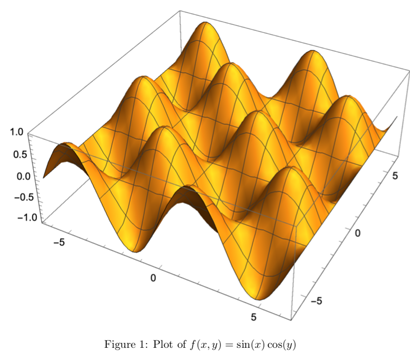
\includegraphics{example.pdf}
%     \caption{Plot of $f(x,y)=\sin(x)\cos(y)$}
%     \centering
%   \end{figure}
% \end{verbatim}
% \begin{figure}[htb]
%   \wolframgraphics{Plot3D[Sin[x]Cos[y],{x,-2Pi,2Pi},{y,-2Pi,2Pi}]}{example}
%   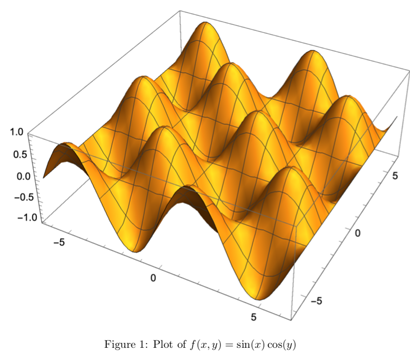
\includegraphics{example.pdf}
%   \caption{Plot of $f(x,y)=\sin(x)\cos(y)$}
%   \centering
%   \label{fig:example}
% \end{figure}
%
% In the \texttt{mathics} mode, plots are exported as \texttt{.asy} files (Asymptote graphics), and the \texttt{asymptote} package\footnote{\url{https://ctan.org/pkg/asymptote}} is required to import the plots. Here is an example:
% \begin{verbatim}
%   \begin{figure}
%     \wolframgraphics{Plot[Sin[x],{x,0,2Pi}]}{example}
%     \input{example.asy}
%   \end{figure}
% \end{verbatim}
%
% Note that you need to process the \texttt{.asy} files so they can be included in the next compilation. For example,
% \begin{verbatim}
%   pdflatex -shell-escape mydocument.tex
%   asy mydocument-*.asy
%   pdflatex -shell-escape mydocument.tex
% \end{verbatim}
%
% Please refer to the documentation of the \texttt{asymptote} package for more information.
% \vspace{15pt}
%
% \DescribeMacro{\wolframalpha}
% \fbox{\texttt{\backslash wolframalpha}\oarg{format}\marg{query}}
% sends a query to Wolfram$\vert$Alpha and put the result into the document. The options for format are \texttt{tex} (default), \texttt{wolfram}, \texttt{wolfram2} and \texttt{text}. The options \texttt{wolfram} and \texttt{wolfram2} correspond to the pure standard Wolfram Language result and the result generated by free-form input, respectively. In the Wolfram Language documutation\footnote{\url{https://reference.wolfram.com/language/ref/WolframAlpha.html}}, the former corresponds to the \texttt{WolframResult} format, and the latter corresponds to the \texttt{Result} format. The default option \texttt{tex} uses the \texttt{WolframResult} format and converts the result into the \TeX~form. Besides, the option \texttt{text} generates plain text which is the result of the \texttt{ShortAnswer} format. As an example,
% \begin{spverbatim}
%   The population of Shanghai is $\wolframalpha{Shanghai population}$, which is $\wolframalpha{ratio of Shanghai population and NYC population}$ times the population of New York City.
% \end{spverbatim}
% \newline
% generates ``The population of Shanghai is $\wolframalpha{Shanghai population}$, which is $\wolframalpha{ratio of Shanghai population and NYC population}$ times the population of New York City.''
% \vspace{15pt}
%
% \DescribeMacro{\wolframsolve}
% \fbox{\texttt{\backslash wolframsolve}\marg{equation}\marg{variable}} solves an equation and display the corresponding results. For example,
% \begin{verbatim}
%   \wolframsolve{a x^2+b x+c==0}{x}
% \end{verbatim}
% produces
% \wolframsolve{a x^2+b x+c==0}{x}
%
% \DescribeMacro{\wolframdsolve}
% \fbox{\texttt{\backslash wolframdsolve}\marg{equation}\marg{dependent variable}\marg{independent variable}} is similar to \texttt{\backslash wolframsolve}, but it solves an differential equation. For example,
% \begin{verbatim}
%   \wolframdsolve{y'[x]+y[x]==a Sin[x]}{y[x]}{x}
% \end{verbatim}
% produces
% \wolframdsolve{y'[x]+y[x]==a Sin[x]}{y[x]}{x}
%
% \DescribeMacro{\wolframtex}
% \fbox{\texttt{\backslash wolframtex}\marg{format}\marg{code}} takes \TeX~code instead of Wolfram Language code, and performs some simple calculations. The options for format are the same as \texttt{\backslash wolfram}, i.e. \texttt{tex} (default), \texttt{wolfram} and \texttt{text}. For example, the result of
% \begin{verbatim}
%   $$ \wolframtex{\int_a^b\sin(x)\,dx} $$
% \end{verbatim}
% is
% $$ \wolframtex{\int_a^b\sin(x)\,dx}. $$
% \vspace{15pt}
%
% \DescribeMacro{\wolframanimation}
% \fbox{\texttt{\backslash wolframanimation}\marg{code}\marg{foldername}} is similar to \texttt{\backslash wolframgraphics}, but it converts any Wolfram Language animation object into a sequence of images, instead of a single image. The images are saved in a subfolder of current folder, named as $\langle\textit{foldername}\rangle$. You can then use \texttt{\backslash animategraphics} from the \texttt{animate} package\footnote{\url{https://ctan.org/pkg/animate}} to generate animation. Note that PDF files with animations can only be viewed in a small number of PDF readers, which includes Acrobat Reader. Please refer to the documentation for the \texttt{animate} package for more information.
% \vspace{15pt}
%
% \DescribeMacro{\wolframtable}
% \fbox{\texttt{\backslash wolframtable}\marg{table}} converts a table in Wolfram Language into \TeX~form. The macro can be put inside environments such as \texttt{tabular}, \texttt{tabularx}, etc. For example,
%
% \begin{verbatim}
%   \begin{center}
%     \begin{tabular}{ccc}
%       \hline
%       \wolframtable{Join[{{x,x^2,x^3}},Table[{i,i^2,i^3},{i,5}]]}
%       \hline
%     \end{tabular}
%   \end{center}
% \end{verbatim}
% generates the following table:
% \begin{center}
%   \begin{tabular}{ccc}
%     \hline
%     \wolframtable{Join[{{x,x^2,x^3}},Table[{i,i^2,i^3},{i,5}]]}
%     \hline
%   \end{tabular}
% \end{center}
%
% \subsection{Notes}
% \begin{enumerate}
%   \item If you want to input backslashs (\texttt{\backslash}) or number signs (\texttt{\hash}) in your Wolfram Language codes, you could use \texttt{\backslash backslash} and \texttt{\backslash hash}, respectively. For example, use \texttt{\backslash backslash[Alpha]} instead of \texttt{\backslash [Alpha]} to represent the Greek letter $\alpha$.
%   \item Outputs are cached in hidden files named as $\texttt{.latexalpha2\char`\_}\langle hash\rangle\texttt{.out}$, unless the option \texttt{nocache} is specified. You can clean the cached outputs manually using the following command if you like:
%     \begin{verbatim}
%       rm .latexalpha2_*.out
%     \end{verbatim}
%   \item \texttt{\backslash def} could be utilized to create re-useable code snippets. For example,
%     \begin{verbatim}
%       \def\mat{{{a,b},{c,d}}}
%       $$ \wolfram{\mat}^{-1} = \wolfram{Inverse[\mat]}. $$
%     \end{verbatim}
%     generates
%     \def\mat{{{a,b},{c,d}}}
%     $$ \wolfram{\mat}^{-1} = \wolfram{Inverse[\mat]}. $$
% \end{enumerate}
%
% \section{Acknowledgement}
%
% This package is heavily inspired by \texttt{LaTeX-Alpha}\footnote{\url{https://github.com/Akollek/LaTeX-Alpha}}, which also explains the name of this package. Unfortunately, \texttt{LaTeX-Alpha} has been down for a while. The objective of this package is to replace \texttt{LaTeX-Alpha} and at the same time provide various new features.
%
% \StopEventually{}
%
% \section{Implementation}
%
%    \begin{macrocode}
%
\RequirePackage{graphicx}
\RequirePackage{amsmath}
\RequirePackage{etoolbox}
\RequirePackage{pdftexcmds}
\RequirePackage{morewrites}
\RequirePackage{ifxetex}

\newbool{ifcache}
\newbool{ifmathics}

\DeclareOption{local}{\def\la@platform{-local}}
\DeclareOption{cloud}{\def\la@platform{-cloud}}
\DeclareOption{cache}{\booltrue{ifcache}}
\DeclareOption{nocache}{\boolfalse{ifcache}}
\DeclareOption{mathics}{\booltrue{ifmathics}}

\ExecuteOptions{local,cache}
\ProcessOptions\relax

\begingroup
  \makeatletter
  \catcode`#=12
  \catcode`&=12
  \gdef\@hashchar{#}
  \gdef\@ampchar{&}
  \gdef\backslash{\@backslashchar}
  \gdef\hash{\@hashchar}
  \makeatother
\endgroup

\def\la@codetempfile{latexalpha2_code.tmp}
\def\la@resulttempfile{}
\def\la@currcodehash{}

\newcommand{\la@cleancodetempfile}{\immediate\write18{rm -f \la@codetempfile}}
\newcommand{\la@unknownoption}[2]{\PackageError{latexalpha2}{Unknown option '#2' for \@backslashchar #1}{}}

\newcommand{\la@executewolfram}[1]{%
  \IfFileExists{\la@resulttempfile}{%
    \ifbool{ifcache}{\message{found cached output file \la@resulttempfile^^J}}{\la@executewolframcore{#1}}%
  }{\la@executewolframcore{#1}}%
}

\newcommand{\la@executewolframcore}[1]{%
  \notbool{ifmathics}{%
    \def\la@wolframscript{wolframscript -file \la@codetempfile\space -print \ifblank{#1}{}{-format #1} \la@platform\space> \la@resulttempfile}%
  }{%
    \def\la@wolframscript{mathics \la@codetempfile\space> \la@resulttempfile}%
  }%
  \message{command: \la@wolframscript^^J}%
  \immediate\write18{\la@wolframscript}%
}

\newcommand{\la@writecodefile}[2]{%
  \message{------------ latexalpha2 -------------^^J}%
  \message{\notbool{ifmathics}{wolfram}{mathics} code: #1^^J}%
  \ifblank{#2}{}{\message{option: #2}}%
  \gdef\la@currcodehash{\ifxetex\mdfivesum{#1#2}\else\pdfmdfivesum{#1#2}\fi}%
  \gdef\la@resulttempfile{.latexalpha2_\la@currcodehash.out}%
  \newwrite\tempfile%
  \immediate\openout\tempfile=\la@codetempfile%
  \immediate\write\tempfile{#1}%
  \immediate\closeout\tempfile%
}

\newcommand{\la@notformathics}[1]{%
  \ifbool{ifmathics}{\PackageError{latexalpha2}{\@backslashchar #1 is not available for the Mathics mode}{}}{}%
}

\def\la@texformat{tex}
\def\la@textformat{text}
\def\la@wolframformat{wolfram}
\def\la@wolframtwoformat{wolfram2}
\def\la@pdfformat{pdf}
\def\la@pngformat{png}
\def\la@jpgformat{jpg}

%^^A [<format>]{<code>}
\newcommand{\wolfram}[2][tex]{%
  \def\la@currformat{#1}%
  \la@cleancodetempfile%
  \notbool{ifmathics}{%
    \la@writecodefile{#2}{#1}%
    \ifx \la@currformat \la@texformat \la@executewolfram{TeXForm} \else
    \ifx \la@currformat \la@textformat \la@executewolfram{Text} \else
    \ifx \la@currformat \la@wolframformat \la@executewolfram{} \else
    \la@unknownoption{wolfram}{#1}
    \fi\fi\fi
  }{%
    \ifx \la@currformat \la@texformat \la@writecodefile{Print[TeXForm[#2]]}{#1} \else
    \ifx \la@currformat \la@wolframformat \la@writecodefile{Print[#2]}{#1} \else
    \la@unknownoption{wolfram}{#1}
    \fi\fi
    \la@executewolfram{}
  }
  \input{\la@resulttempfile}%%
  \la@cleancodetempfile%
}

%^^A [<format>]{<code>}
\newcommand{\wolframalpha}[2][tex]{%
  \la@notformathics{wolframalpha}%
  \def\la@currformat{#1}%
  \la@cleancodetempfile%
  \la@writecodefile{WolframAlpha["#2","%
    \ifx\la@currformat\la@textformat ShortAnswer\else
    \ifx\la@currformat\la@wolframtwoformat Result\else
    WolframResult\fi\fi
    "]}{#1}%
  \ifx \la@currformat \la@textformat \la@executewolfram{} \else
  \ifx \la@currformat \la@wolframformat \la@executewolfram{} \else
  \ifx \la@currformat \la@wolframtwoformat \la@executewolfram{} \else
  \ifx \la@currformat \la@texformat \la@executewolfram{TeXForm} \else
  \la@unknownoption{wolframalpha}{#1}
  \fi\fi\fi\fi
  \input{\la@resulttempfile}%
  \la@cleancodetempfile%
}

%^^A [<format>]{<code>}{<filename>}
\newcommand{\wolframgraphics}[3][pdf]{%
  \def\la@currformat{#1}%
  \la@cleancodetempfile%
  \notbool{ifmathics}{%
    \la@writecodefile{#2}{#1}%
    \ifx \la@currformat \la@pdfformat \la@executewolfram{PDF} \else
    \ifx \la@currformat \la@pngformat \la@executewolfram{PNG} \else
    \ifx \la@currformat \la@jpgformat \la@executewolfram{JPEG} \else
    \la@unknownoption{wolframgraphics}{#1}
    \fi\fi\fi
    \ifx \la@currformat \la@pdfformat \immediate\write18{cp\space\la@resulttempfile\space#3.pdf} \else
    \ifx \la@currformat \la@pngformat \immediate\write18{cp\space\la@resulttempfile\space#3.png} \else
    \ifx \la@currformat \la@jpgformat \immediate\write18{cp\space\la@resulttempfile\space#3.jpg} \else
    \la@unknownoption{wolframgraphics}{#1}
    \fi\fi\fi
  }{%
    \la@writecodefile{Print[TeXForm[#2]]}{asy}
    \la@executewolfram{}
    \immediate\write18{cp\space\la@resulttempfile\space#3.asy}
  }
}

%^^A {<equation>}{<variable>}
\newcommand{\wolframsolve}[2]{%
  \la@cleancodetempfile%
  \def\la@solvecode{"\@backslashchar\@backslashchar begin{flalign*}"<>StringJoin@@("\@ampchar"<>ToString[ToExpression["TeXForm"][#2]]<>"="<>ToString[ToExpression["TeXForm"][\@hashchar]]<>"\@backslashchar\@backslashchar\@backslashchar\@backslashchar"\@ampchar/@(#2/.Solve[#1, #2]))<>"\@backslashchar\@backslashchar end{flalign*}"}
  \notbool{ifmathics}{%
    \la@writecodefile{\la@solvecode}{}%
    \la@executewolfram{Text}%
  }{%
    \la@writecodefile{Print[\la@solvecode]}{}%
    \la@executewolfram{}%
  }
  \input{\la@resulttempfile}%
  \la@cleancodetempfile%
}

%^^A {<equation>}{<dependent variable>}{<independent variable>}
\newcommand{\wolframdsolve}[3]{%
  \la@cleancodetempfile%
  \def\la@solvecode{"\@backslashchar\@backslashchar begin{flalign*}"<>StringJoin@@("\@ampchar"<>ToString[ToExpression["TeXForm"][#2]]<>"="<>ToString[ToExpression["TeXForm"][\@hashchar]]<>"\@backslashchar\@backslashchar\@backslashchar\@backslashchar"\@ampchar/@(#2/.DSolve[#1, #2, #3]))<>"\@backslashchar\@backslashchar end{flalign*}"}
  \notbool{ifmathics}{%
    \la@writecodefile{\la@solvecode}{}%
    \la@executewolfram{Text}%
  }{%
    \la@writecodefile{Print[\la@solvecode]}{}%
    \la@executewolfram{}%
  }
  \input{\la@resulttempfile}%
  \la@cleancodetempfile%
}

%^^A {<format>}{<code>}
\newcommand{\wolframtex}[2][tex]{%
  \la@notformathics{wolframtex}%
  \def\la@currformat{#1}%
  \la@cleancodetempfile%
  \la@writecodefile{ToExpression["\unexpanded{#2}", TeXForm]}{#1}%
  \immediate\write18{sed -i '' 's/\@backslashchar\@backslashchar/\@backslashchar\@backslashchar\@backslashchar\@backslashchar/g' \la@codetempfile}%
  \ifx \la@currformat \la@texformat \la@executewolfram{TeXForm} \else
  \ifx \la@currformat \la@textformat \la@executewolfram{Text} \else
  \ifx \la@currformat \la@wolframformat \la@executewolfram{} \else
  \la@unknownoption{wolframtex}{#1}
  \fi\fi\fi
  \input{\la@resulttempfile}%
  \la@cleancodetempfile%
}

%^^A {<code>}{<foldername>}
\newcommand{\wolframanimation}[2]{%
  \la@notformathics{wolframanimation}%
  \la@cleancodetempfile%
  \la@writecodefile{#1}{}%
  \la@executewolfram{GIF} 
  \immediate\write18{cp\space\la@resulttempfile\space#2.gif}%
  \immediate\write18{mkdir -p #2}%
  \immediate\write18{convert -coalesce #2.gif #2/frame.png}%
  \la@cleancodetempfile%
}

%^^A {<table>}
\newcommand{\wolframtable}[1]{%
  \la@notformathics{wolframtable}%
  \la@cleancodetempfile%
  \def\la@tablecode{StringJoin@@((StringRiffle[("$"<>Slot[1]<>"$")\@ampchar/@ToString/@TeXForm/@(Slot[1]),"\space\@ampchar\space"]<>"\@backslashchar\@backslashchar\@backslashchar\@backslashchar")\@ampchar/@(#1))}%
  \la@writecodefile{\la@tablecode}{}%
  \la@executewolfram{Text}%
  \la@cleancodetempfile%
  \input{\la@resulttempfile}%
}

\AtBeginDocument{%
  %^^A check if shell-escape is available
  \ifcase\pdf@shellescape
  \PackageError{latexalpha2}{Shell escape is not enabled, which is required to use latexalpha2}{}\or
  \PackageInfo{latexalpha2}{Shell escape is successfully enabled}{}\or
  \PackageError{latexalpha2}{Shell escape is not enabled, which is required to use latexalpha2}{}\fi

  %^^A check if wolframscript or mathics is available
  \immediate\write18{command -v \notbool{ifmathics}{wolframscript}{mathics}; echo $? > latexalpha2_check.tmp}%
  \newread\wsreturncodefile%
  \immediate\openin\wsreturncodefile=latexalpha2_check.tmp%
  \readline\wsreturncodefile to \wsreturncode%
  \immediate\closein\wsreturncodefile%
  %^^A https://tex.stackexchange.com/a/26873
  \def\instring#1#2{TT\fi\begingroup\edef\x{\endgroup\noexpand\in@{#1}{#2}}\x\ifin@}%
  \notbool{ifmathics}{%
    \if\instring{0}{\wsreturncode}
    \PackageInfo{latexalpha2}{WolframScript is available}{}\else
    \PackageError{latexalpha2}{WolframScript cannot be found, which is required to use latexalpha2}{}\fi
  }{%
    \if\instring{0}{\wsreturncode}
    \PackageInfo{latexalpha2}{Mathics is available}{}\else
    \PackageError{latexalpha2}{Mathics cannot be found, which is required to use the Mathics mode of latexalpha2}{}\fi
  }
}

\AtEndDocument{%
  \ifbool{ifcache}{}{\immediate\write18{rm -f .latexalpha2_*.out}}
}
%    \end{macrocode}
%
% \Finale
%
\endinput
